\section{Electrons in a Periodic Potential: Band Theory of Solids}

\subsection{Review: Bloch's Theorem}
See A\&M Ch. 8 for proof(s) and extended discussion.

\textbf{Theorem (Bloch).} Consider the eigenstates $\psi$ of the one-electron Hamiltonian:
\begin{align*}
    H = \frac{\hbar^2\nabla^2}{2m} + U(\v{r})
\end{align*}
where $U(\v{r} + \v{R}) = U(\v{r})$ for all $\v{R}$ in the Bravais lattice. These eigenstates can be chosen to have the form:
\begin{equation}\label{eq-Blocheigenstates}
    \boxed{\psi_{nk}(\v{r}) = e^{i\v{k}\cdot \v{r}}\mu_{nk}(\v{r})}
\end{equation}
where:
\begin{equation}\label{eq-Blocheigenstatesperiodic}
    \mu_{nk}(\v{r} + \v{R}) = \mu_{nu}(\v{r})
\end{equation} 

The interesting part of this statement is that even though the Haniltonian has a full symmetry under translation by $+ \v{R}$. The eigenstates do not; there is a part that possesses the symmetry $\mu_{nk}(\v{r})$ and a part that does not, $e^{i\v{k} \cdot \v{r}}$ which is translation invariant. This should not be totally unexpected; for example the QHO is symmetric under inversion, but the wavefunctions do not have all of this symmetry ($n$ even is even, $n$ odd is odd).

A remark: Note that Eqs. \eqref{eq-Blocheigenstates} and \eqref{eq-Blocheigenstatesperiodic} imply that:
\begin{equation}
    \psi_{nk}(\v{r} + \v{R}) = e^{i\v{k} \cdot \v{R}}\psi_{nk}(\v{r}).
\end{equation}

In Eq. \eqref{eq-Blocheigenstates}, $\v{k}$ is known as a crystal momentum and $n$ is the band index. In free space, complete translation invariance implies the conservation of momentum. In a lattice, we have translation invariance w.r.t the Bravais lattice $\v{R}$, only, which implies that momentum is not conserved, but the crystal momentum is conserved.

\subsection{Weak Periodic Potential}
This is also known as ``nearly free'' electrons in a periodic lattice. We consider the same Hamiltonian $H = \frac{\hbar^2\nabla^2}{2m} + U(\v{r})$ where $U(\v{r})$ is ``weak'', sufficiently weak enough to be treated in perturbation theory. We call $H_0 = \frac{\hbar^2\nabla^2}{2m}$ and $H' = U(\v{r})$.

First, we transform $H$ into second-quantized notation:
\begin{equation}
    \begin{split}
        H_0 &= \sum_{\v{k}, \sigma} \e_\v{k}c^\dag_{\v{k}\sigma}c_{\v{k}\sigma}, \quad \e_\v{k} = \frac{\hbar^2\v{k}^2}{2m}
        \\ H' &= \sum_{\v{k}\v{k}'\sigma\sigma'}\bra{\v{k}\sigma}U\ket{\v{k}'\sigma}c_{\v{k}\sigma}^\dag c_{\v{k}'\sigma'}
    \end{split}
\end{equation}
where we note that as usual we work in the plane wave basis $\psi_\v{k} = \frac{1}{\sqrt{V}}e^{i\v{k} \cdot \v{r}}$, and so:
\begin{equation}
    \sum_{\v{k}\v{k}'\sigma\sigma'}\bra{\v{k}\sigma}U\ket{\v{k}'\sigma} = \frac{1}{V}\delta_{\sigma\sigma'}\int d^3 r e^{-i\v{r}\cdot(\v{k} - \v{k}')}U(\v{r})
\end{equation}
Note that due to its periodic property, $U$ can be written as:
\begin{equation}
    U(\v{r}) = \sum_{\v{G}}e^{i\v{r} \cdot \v{G}}U_\v{G}
\end{equation}
where $\v{G}$ are reciprocal lattice vectors satisfying $e^{i\v{G} \cdot \v{R}} = 1$ for all $\v{R}$ in the Bravais lattice (check)! $U_\v{G}$ is the fourier transform of our potential, evaluated at $\v{G}$.

We further assume that $U_{\v{G} = 0} = 0$, which only redefines the overall energy zero. We can therefore write:
\begin{equation}
    \bra{\v{k}\sigma}U\ket{\v{k}'\sigma'} = \frac{\delta_{\sigma\sigma'}}{V} \int d^3r \sum_\v{G} U_\v{G} e^{-i\v{r}\cdot(\v{k} - \v{k'} - \v{G})} = \delta_{\sigma\sigma'}\sum_\v{G}U_\v{G}\delta_{\v{k} - \v{k}', \v{G}}
\end{equation}
when the dust settles, we find:
\begin{equation}
    H' = \sum_{\v{k}\v{G}\sigma} U_\v{G} c^\dag_{\v{k} + \v{G}\sigma}c_{\v{k}\sigma}
\end{equation}
which is a very suggestive rewrite; for each term corresponds to the destruction of an electron with wavevector $\v{k}$ and the creation of an electron with wavevector $\v{k} + \v{G}$. This also explains the conservation of crystal momentum; the electron undergoes scattering processes which changes the momentum from $\v{k}$ to $\v{k} + \v{G}$ (so momentum is not conserved) but the crystal momentum (i.e. momentum up to reciprocal lattice vectors) is. This also connects back to the Bruillion zone; the wavevector $\v{k}$ appearing here can always be confined to the first Bruillion zone.

In the following, we suppress the spin index, and focus on 1D systems for simplicity. So, we have:
\begin{align*}
    H_0 = \sum_k \e_k c^\dag_k c_k, \quad H' = \sum_{k, G} U_G c^\dag_{k + G}c_k
\end{align*}
we ask how is an electron in an eigenstates $\ket{k} = c^\dag_k \ket{0}$ of $H_0$ perturbed by $H'$.

\subsubsection{Zeroth-order perturbation theory}
To start, in zeroth order perturabtion theory, we have:
\begin{equation}
    E_k^{(0)} = \e_k
\end{equation}
Of course, nothing exciting here...

\subsubsection{First-order perturbation theory}
We have:
\begin{equation}
    E_k^{(1)} = \bra{k}H'\ket{k} = \bra{k}\sum_{q,G} U_G c^\dag_{q + G}c_q\ket{k} = \bra{k}\sum_G U_G c_{k+G}^\dag \ket{0} = \sum_G U_G\braket{k}{k+G} = U_0 = 0.
\end{equation}
so the first order contribution is zero.

\subsubsection{Second-order perturbation theory}
We have:
\begin{equation}
    E_k^{(2)} = \sum_{k' \neq k} \frac{\abs{\bra{k}H'\ket{k'}}^2}{\e_{k'} - \e_k}
\end{equation}
So we calculate:
\begin{equation}
    \bra{k}H'\ket{k'} = \sum_{qG}U_G\bra{k}c^\dag_{q + G}c_q \ket{k'} = \sum_G U_G\bra{k}c^\dag_{k'+G}\ket{0} = \sum_G U_G\braket{k}{k'+G} = \sum_G U_G \delta_{k, k'+G} = 
\end{equation}
Therefore:
\begin{equation}
    E_k^{(2)} = \sum_{k' \neq k, G, G'}\frac{U_G U_{G'}^* \delta_{k,k'+G}\delta_{k, k'+G'}}{\e_{k'} - \e_k} = \sum_{G \neq 0,G'} \frac{U_G U_{G'}^* \delta_{GG'}}{\e_{k+G} - \e_k} = \sum_{G \neq 0} \frac{\abs{U_G}^2}{\e_{k+G} - \e_k}
\end{equation}

For small $\abs{U_G}$, this correction is small, EXCEPT when $\abs{\e_{k - G} - \e_k}$ is also small. This occurs at specific values of $\v{k} = \frac{1}{2}\v{G}$ (valid also in 3D). However this is not the final answer; in reality there will not be an infinite correction. What's the catch? When we do perturbation theory as we have, we assume that the energy levels are non-degenerate; but here there is a degeneracy. Hence, at and near $\v{k} = \frac{1}{2}\v{G}$, we must apply degenerate perturbation theory because $\e_{k - G} = \e_k$ and this could be viewed as a degeneracy.

\subsection{Degenerate Perturbation Theory}
We define two near degenerate states:
\begin{equation}
    \ket{1} = \ket{k}, \quad \ket{2} = \ket{k - G_1}
\end{equation}
and construct the Hamiltonian matrix in this basis:
\begin{equation}
    H = \m{\bra{1}H\ket{1} & \bra{1}H\ket{2} \\ \bra{2}H\ket{1} & \bra{2}H\ket{2}} = \m{\e_k & U_G \\ U_G^* & \e_{k-G}}
\end{equation}
The perturbed energies are given by eigenvalues:
\begin{equation}
    \det\m{\e_k - E & U_G \\ U_G^* & \e_{k-G} - E} = 0 \implies (\e_k - E)(\e_{k-G} - E) - \abs{U_G}^2 = 0
\end{equation}
so then:
\begin{equation}
    E_k = \frac{1}{2}\left(\e_k + \e_{k-G}\right) \pm \sqrt{\frac{1}{4}\left(\e_k - \e_{k-G}\right)^2 + \abs{U_G}^2}
\end{equation}
Note for $k = \frac{1}{2}G$, i.e. the degeneracy point, this implies:
\begin{equation}
    E_k = \e_k \pm \abs{U_G}.
\end{equation}
So we have an energy gap! This quantifies the distinction of metals and insulators, using quantum mechanics; we will go further into this discussion next class.

\begin{figure}[htbp]
    \centering
    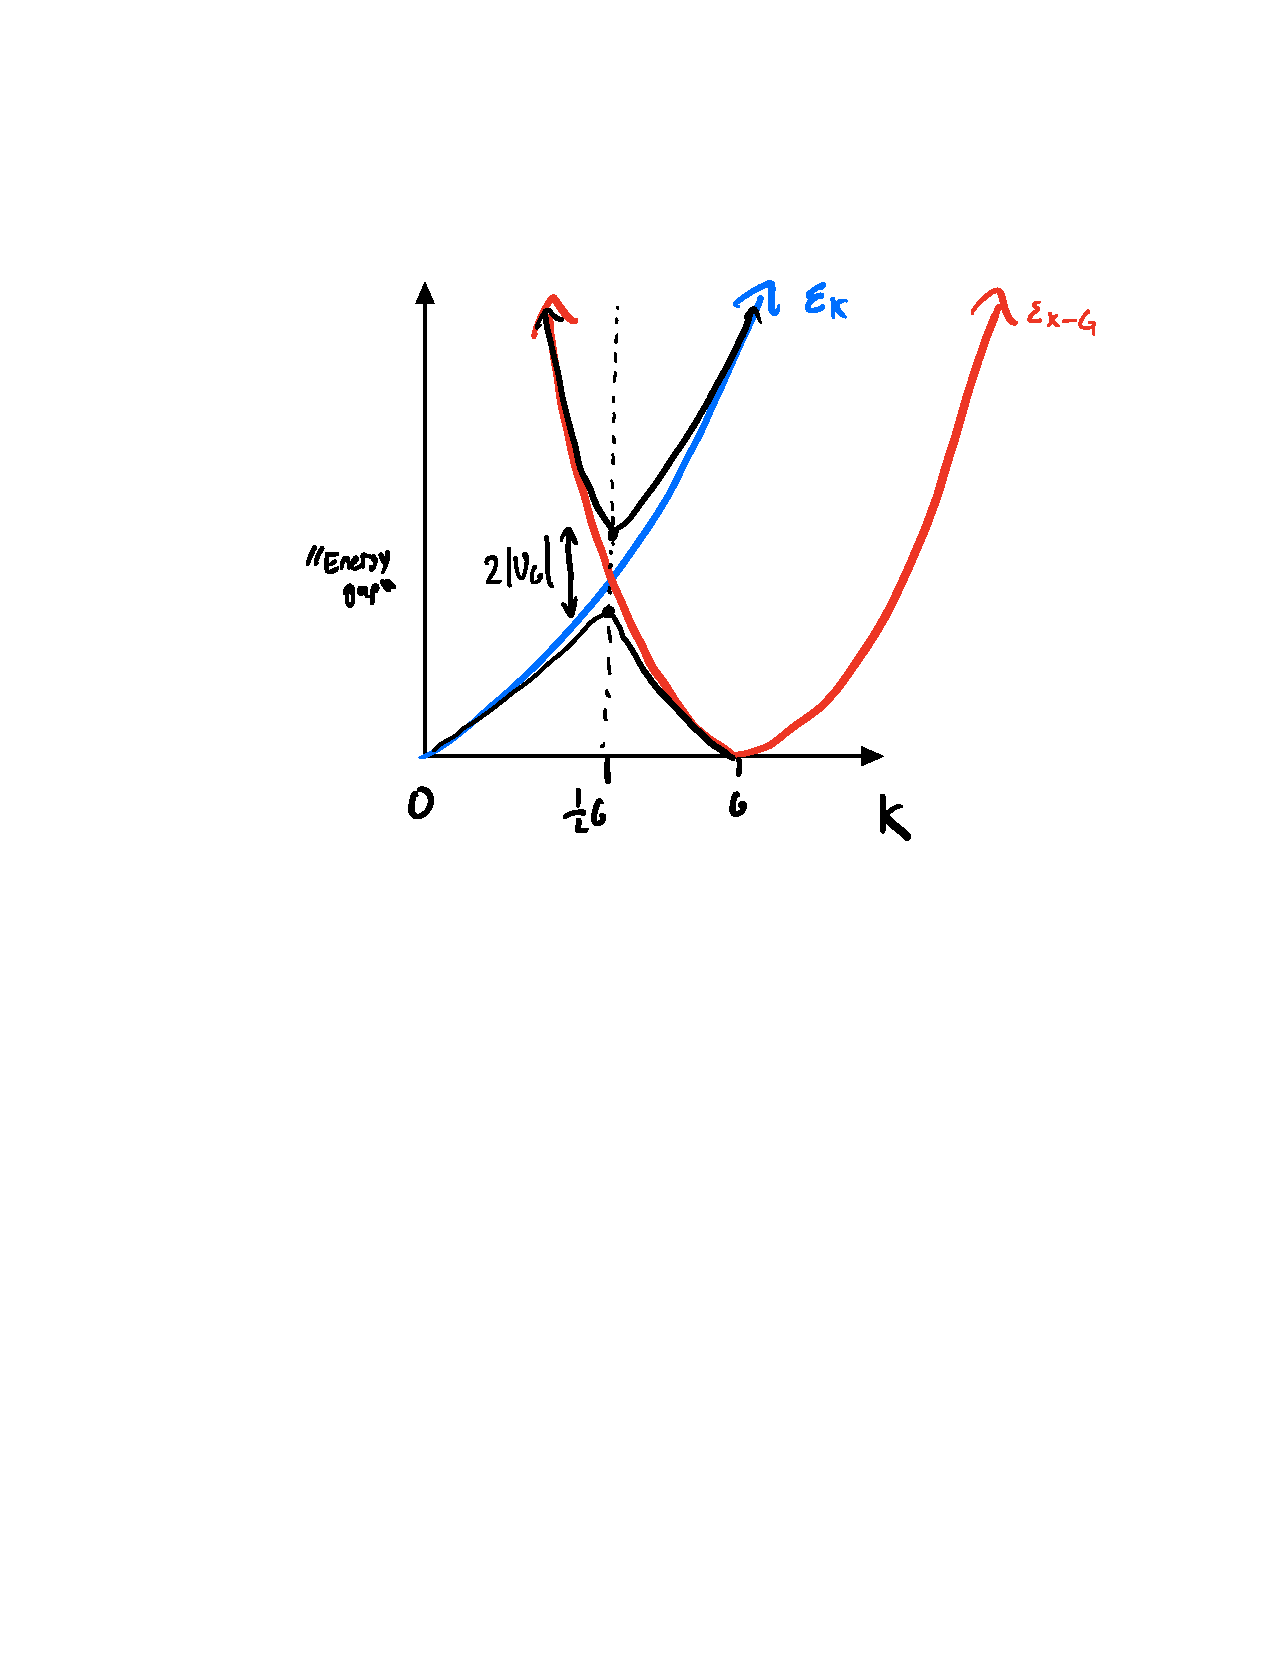
\includegraphics[scale=0.7]{Images/fig-energyvskgap.pdf}
    
    \caption{Plot of the energy $\e_k$ and $\e_{k-G}$ as a function of $k$. At $k = \frac{1}{2}G$ the two energy functions coincide. At and near this point, non-degenerate perturbation theory breaks down. A more careful treatment using degenerate perturbation theory shows that there are two energy levels, separated by a gap $2\abs{U_G}$.}
    \label{fig-energyvskgap}
\end{figure}